
\section{HAR en Android}
\begin{frame}{Proyecto HARDroid}

\framesubtitle{HAR en Android}

\setbeamercovered{transparent}
\begin{columns}

\column{0.4\textwidth}
\begin{itemize}
\item \textbf{HARDroid} 
\begin{itemize}
\item Servicio utilitario de reconocimiento.
\item Clasificador din�mico
\end{itemize}
\begin{spacing}{0.5}

\pause{}
\end{spacing}
\item \textbf{ActivitySurvey}
\begin{itemize}
\item Aplicaci�n que depende del servicio.
\item Encuesta a usuarios. 
\end{itemize}
\begin{spacing}{0.5}

\pause{}
\end{spacing}
\item \textbf{Backend C4.5} 
\begin{itemize}
\item Servicio web de recolecci�n.
\item Aciertos son utilizados para mejorar el clasificador.
\end{itemize}
\end{itemize}

\column{0.6\textwidth}
\begin{center}
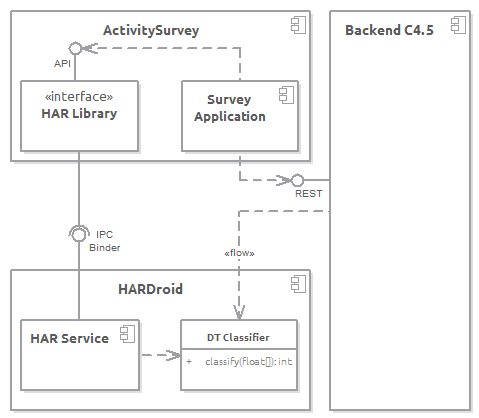
\includegraphics[width=1\columnwidth]{propuesta/graphics/arqui_general}
\par\end{center}

\end{columns}

\end{frame}
%

